\documentclass[conference]{IEEEtran}
\IEEEoverridecommandlockouts

\usepackage{amsmath,amssymb}
\usepackage{graphicx}
\usepackage{booktabs}
\usepackage{hyperref}
\usepackage{float}
\usepackage{array}

\hyphenation{op-tical net-works semi-conduc-tor}

\begin{document}

\title{PHC Integrated Digital System for IIT Jodhpur:\\
Solution Trajectory, Implementation Results, and Current Status}

\author{
\IEEEauthorblockN{Bavadiya Yash Kiritbhai}
\IEEEauthorblockA{B24CS1019}
\and
\IEEEauthorblockN{Chaitanya Singh}
\IEEEauthorblockA{B24CS1088}
\and
\IEEEauthorblockN{Nayan Patidar}
\IEEEauthorblockA{B24CS1047}
}

\maketitle

\begin{abstract}
This report presents the Assignment 2 status of the PHC Integrated Digital System being developed for the Primary Health Centre at IIT Jodhpur. The project targets a campus-scale healthcare environment where patient registration, visit handling, prescriptions, laboratory requests, pharmacy billing, attendance monitoring, and administrative reporting were historically fragmented across paper records and disconnected manual processes. Building on the earlier SRS and UML work, the current implementation has converged on a modular Node.js and Express backend backed by PostgreSQL through Prisma, with role-based access control, JWT session handling, local LDAP-backed authentication for development, QR-assisted check-in, visit-linked traceability, and an expanding automated testing workflow. The report documents the problem motivation, the evolution of the solution from successive SRS refinements, the sprint and Alpha-driven development process, the finalized architectural choices, and the results observed from the working backend. It also records negative findings and operational constraints, including frontend incompleteness, production-readiness gaps, and documentation synchronization drift. The intent is to present not only what the team planned, but what the repository demonstrably achieves as of April 5, 2026.
\end{abstract}

\begin{IEEEkeywords}
Healthcare Information Systems, PHC Digitization, QR Check-in, RBAC, Visit Traceability, Agile Scrum, Prisma, PostgreSQL.
\end{IEEEkeywords}

\section{Problem Statement}
\subsection{Objective and Motivation}
The IIT Jodhpur Primary Health Centre (PHC) serves a bounded but operationally complex campus population of students, faculty, and staff. In its manual form, the PHC workflow suffers from four persistent problems:
\begin{itemize}
    \item \textbf{Fragmented records:} patient history, prescriptions, and reports are difficult to connect longitudinally when stored across physical files.
    \item \textbf{High reception latency:} repeated demographic lookup and visit registration increase waiting time for every walk-in.
    \item \textbf{Low operational visibility:} doctor availability, attendance, and downstream pharmacy or lab status are not visible in real time.
    \item \textbf{Weak traceability:} the consultation, prescription, laboratory, and billing artifacts of a single encounter are not reliably tied together.
\end{itemize}

The objective of the PHC Integrated Digital System is therefore to digitize the entire outpatient lifecycle, from authentication and patient identification to consultation closure and administrative reporting. The system is intended to remain small enough for institutional deployment while still enforcing medical-data discipline comparable to larger healthcare information systems.

The motivation is practical rather than purely academic. The team sought a system that can reduce manual overhead at the reception desk, ensure controlled access to sensitive records, and preserve a single visit-linked source of truth for every medical interaction. The project also had to fit the operating realities of an institute PHC: campus identity infrastructure, limited deployment complexity, a small development team, and the need for iterative validation.

\section{Solution Trajectory}
\subsection{Evolution from Assignment 1 and SRS Iterations}
Assignment 1 captured the project mainly as a design and planning exercise. At that stage, the emphasis was on SRS stabilization, UML modeling, and architectural justification. The current repository shows the transition from that conceptual baseline to a largely implemented backend.

The solution trajectory can be summarized through the main design decisions that survived refinement:
\begin{itemize}
    \item \textbf{SRS 1.x to 2.2:} the requirements matured from a broad PHC idea to a scoped outpatient system with explicit REQ identifiers, role boundaries, sprint logic, and later testing / validation refinement.
    \item \textbf{Document-centric ideas to relational enforcement:} earlier ideation explored more flexible storage options, but the final architecture adopted PostgreSQL so that visit-linked integrity could be guaranteed through relations rather than convention.
    \item \textbf{Module pruning:} non-core ideas such as ambulance-related scope were removed, allowing the system to focus on the PHC's highest-frequency workflows.
    \item \textbf{Visit-centric linkage:} the SRS concept of a unique VisitID matured in implementation as a visit-centered relational backbone in Prisma. Prescriptions, lab requests, bills, vitals, and documents now attach to a specific visit record.
    \item \textbf{Operational differentiation of doctors:} the design retained the distinction between \textit{SPECIALIST} and \textit{PHYSICIAN}, supporting both scheduled and walk-in driven interactions.
\end{itemize}

This trajectory matters because the repository does not merely mirror the wording of the SRS. It reflects the points where the team had to refine, simplify, or formalize the original ideas so they could be implemented without losing traceability or maintainability.

\subsection{Finalized Tech Stack and Architectural Direction}
The current technical direction is a layered modular monolith. This was an intentional decision. A microservices architecture would have added deployment and coordination overhead that is difficult to justify for a single-campus PHC.

\begin{table}[H]
\centering
\caption{Finalized Technology Stack}
\begin{tabular}{|p{2.1cm}|p{5.2cm}|}
\hline
\textbf{Layer} & \textbf{Technology Choice} \\
\hline
Frontend & React + Vite (currently minimal scaffold only) \\
\hline
Backend & Node.js + Express (ESM) \\
\hline
Database & PostgreSQL \\
\hline
ORM & Prisma with generated client \\
\hline
Authentication & JWT sessions; local LDAP-backed bind flow for development, institutional LDAP alignment planned for deployment \\
\hline
Security / Infra & Helmet, CORS controls, role-gated routes, Linux deployment target \\
\hline
Testing & Bruno collection, shell-based smoke suite, CSV result ledger \\
\hline
\end{tabular}
\label{tab:stack}
\end{table}

The architectural pattern followed consistently in the backend is:
\[
\texttt{route} \rightarrow \texttt{controller} \rightarrow \texttt{service} \rightarrow \texttt{Prisma}
\]

This discipline is valuable in an academic project because it makes responsibility boundaries explicit. The controllers remain thin, the services hold validation and business rules, and Prisma is the persistence boundary. Such separation reduces the chance that future frontend work or later Sprint 5 integrations will require invasive rewrites.

\begin{figure}[H]
\centering
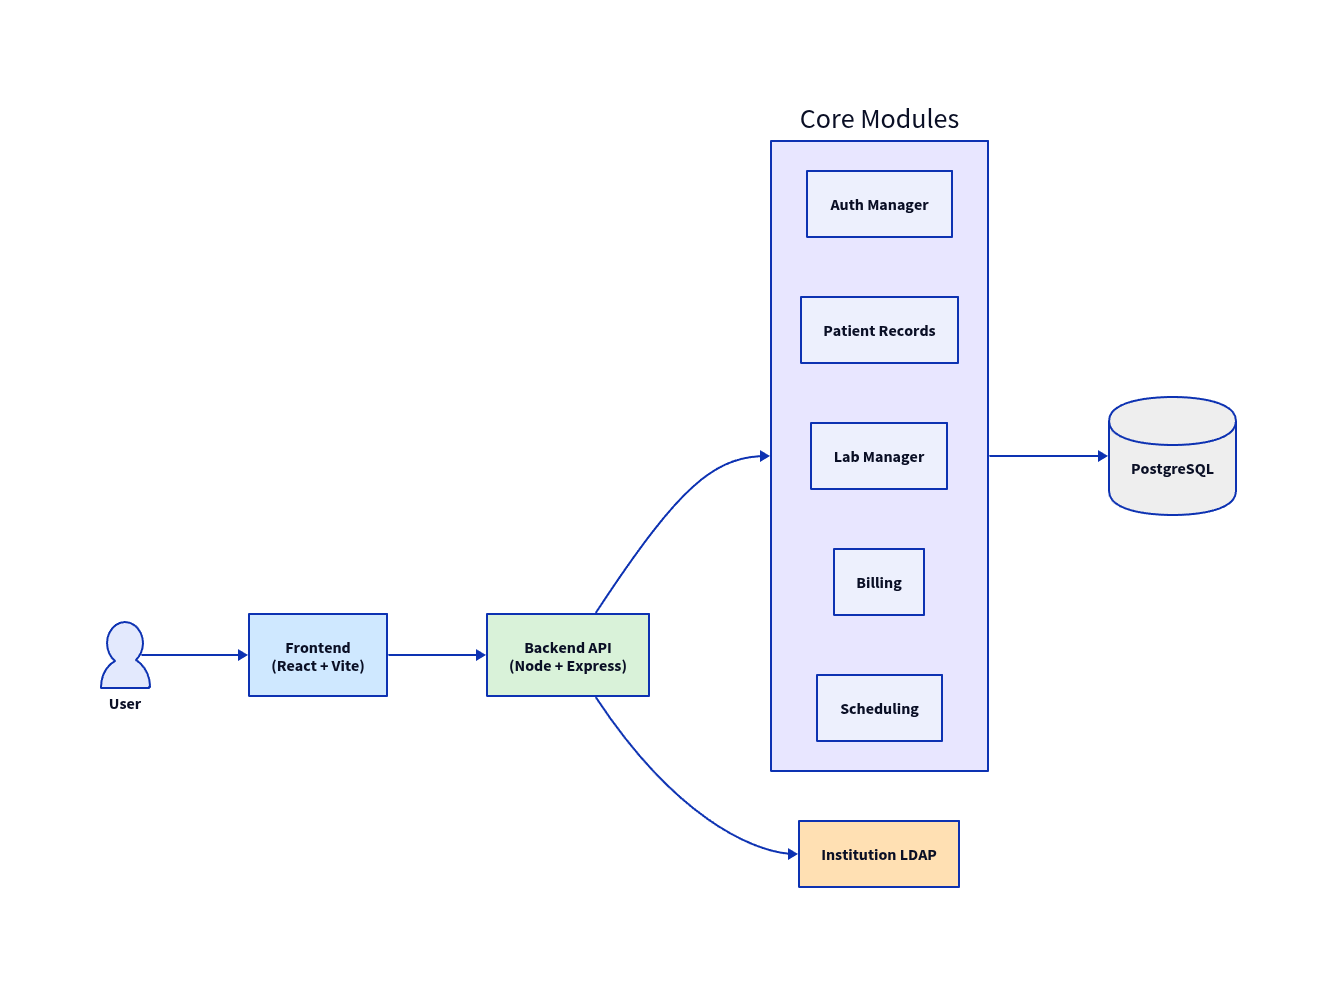
\includegraphics[width=\columnwidth]{figures/phc-system-architecture.png}
\caption{Overall PHC system architecture retained from the SRS/Assignment 1 design baseline and still aligned with the current backend implementation.}
\label{fig:architecture}
\end{figure}

\subsection{Protocols, Algorithms, and Methodology Finalized}
The project does not depend on one mathematically novel algorithm; instead, its value lies in selecting appropriate operational mechanisms and enforcing them consistently.

\subsubsection{Authentication and Access Protocol}
The finalized access model uses JWT for session continuity and role-based authorization at route level. The repository now includes a Dockerized local LDAP server seeded with PHC test users, and authentication is performed through LDAP bind rather than the earlier fallback-only development stub. This is an important implementation correction after Assignment 1 because it moves authentication behavior closer to the intended institutional model. The remaining gap is not local auth correctness, but production-grade alignment with institute infrastructure, deployment hardening, and operational secret handling.

\subsubsection{Visit-Centric Traceability Model}
The central methodology choice is to treat the visit as the anchor of all clinical artifacts. A visit progresses through states such as \texttt{WAITING}, \texttt{IN\_CONSULTATION}, \texttt{COMPLETED}, and \texttt{CANCELLED}. Once this state machine exists, prescriptions, lab requests, bills, and vitals no longer float as isolated records.

\begin{figure}[H]
\centering
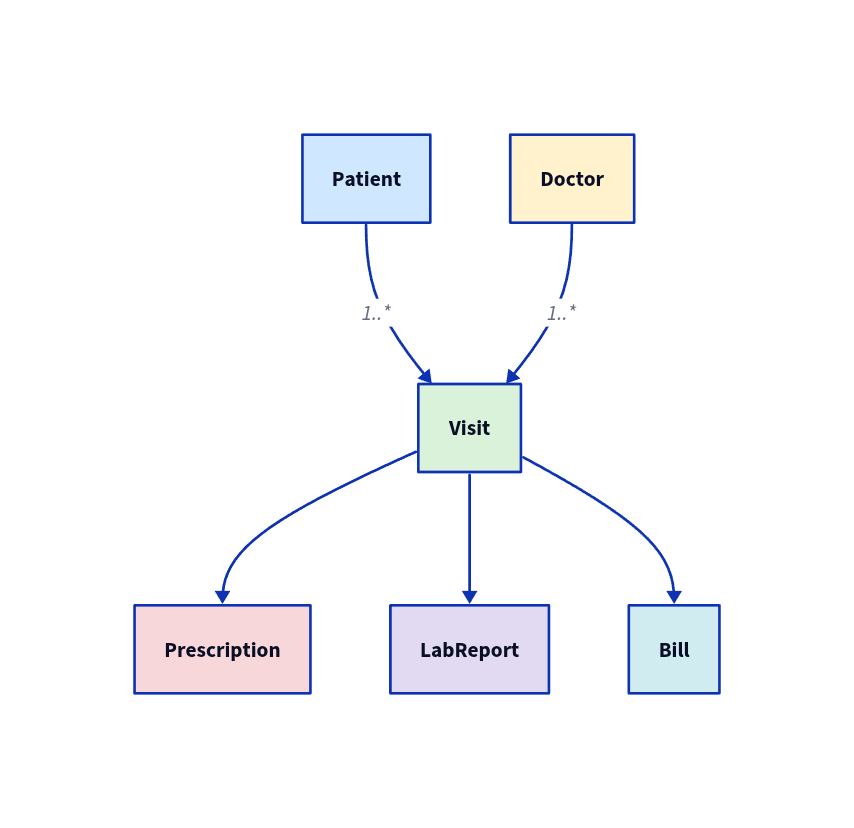
\includegraphics[width=\columnwidth]{figures/visitid-relational-model.png}
\caption{Visit-centric relational design linking clinical, laboratory, and billing entities.}
\label{fig:visitid}
\end{figure}

\subsubsection{Atomic Operations}
Two important implementation choices show methodological maturity beyond the initial report:
\begin{itemize}
    \item \textbf{Billing transaction:} bill creation and stock deduction are executed atomically using \texttt{prisma.\$transaction([...])}.
    \item \textbf{QR check-in composition:} patient resolution, visit creation, and optional vitals insertion occur as one logical check-in operation.
\end{itemize}

These are small but significant examples of where the implementation moves from ``feature present'' to ``feature defensible under failure conditions''.

\subsubsection{Agile / Scrum Execution}
The SRS defines Agile development with short sprints, Trello-based work management, and Essence Alpha ownership. The repository history and documentation indicate that this process was not treated as a formality; it influenced both the module ordering and the re-scoping of later work.

\subsection{Sprint Plan, Scrum Team, and Alpha Progression}
The project is being executed by a three-member Scrum-style team with shared implementation responsibility and Alpha ownership used as an accountability model. From SRS 2.0, the Alpha mapping is as follows.

\begin{table}[H]
\centering
\caption{Essence Alpha Ownership}
\begin{tabular}{|p{2cm}|p{4cm}|}
\hline
\textbf{Alpha} & \textbf{Responsible Member} \\
\hline
Stakeholders, Opportunity, Work & Chaitanya Singh \\
\hline
Software System, Team & Yash Bavadiya \\
\hline
Requirements, Way of Working & Nayan Patidar \\
\hline
\end{tabular}
\label{tab:alpha}
\end{table}

The original SRS proposed five implementation sprints, but the repository's current planning view extends this into seven execution slices, with frontend and stabilization separated. This is a useful example of theory being corrected by implementation reality.

\begin{table}[H]
\centering
\caption{Observed Sprint Status on April 5, 2026}
\begin{tabular}{|p{1.2cm}|p{4.5cm}|p{1.6cm}|}
\hline
\textbf{Sprint} & \textbf{Focus} & \textbf{Status} \\
\hline
0 & SRS, initial UML, schema framing & Complete \\
\hline
1 & Auth, infrastructure, patient profile & Complete \\
\hline
2 & Visit lifecycle, doctor attendance and availability & Complete \\
\hline
3 & Prescription and laboratory modules & Complete \\
\hline
4 & Inventory, billing, appointments, QR check-in, documents & Complete \\
\hline
5 & Admin users, events, reports, notifications, LDAP, integration work & Complete \\
\hline
6 & React dashboards and UX integration & Not started \\
\hline
7 & Hardening, testing, deployment & Not started \\
\hline
\end{tabular}
\label{tab:sprints}
\end{table}

Alpha progression is also visible across the project phases:
\begin{itemize}
    \item \textbf{Stakeholders and Opportunity:} strongest during early PHC workflow study and problem framing.
    \item \textbf{Requirements and Software System:} dominant during SRS refinement and UML convergence.
    \item \textbf{Work and Way of Working:} dominant in the current phase, visible through route-by-route delivery, test scripting, and repository conventions.
    \item \textbf{Team:} increasingly important now that integration, frontend backlog, and documentation synchronization are becoming coordination problems rather than pure design problems.
\end{itemize}

\subsection{Constraints, Limitations, and Challenges Identified}
Several constraints that were abstract in the SRS now appear concretely in the repository:
\begin{itemize}
    \item \textbf{Institutional auth remains a deployment concern:} local LDAP-backed development is working, but campus-grade deployment integration and operational secrets management still need validation.
    \item \textbf{Frontend lag:} the backend has become substantial, but the frontend still contains only a minimal React placeholder screen.
    \item \textbf{Documentation drift:} \texttt{TESTING.md}, \texttt{smoke\_test.sh}, and \texttt{test\_cases.csv} do not all reflect the same current test count, showing that maintenance of secondary artifacts is now a real project risk.
    \item \textbf{Campus-network assumptions:} the SRS assumes a stable institutional network and browser/mobile availability, but no offline mode exists.
    \item \textbf{Incremental scope pressure:} the shift from a five-sprint framing to a seven-sprint README plan reflects the practical need to separate backend completion from frontend delivery and final stabilization.
\end{itemize}

\subsection{Final UML and Structural Baseline}
The final UML baseline used for this report is the same set that emerged from SRS 2.0 and was carried into Assignment 1. This remains a valid choice because the current backend implementation still aligns with those diagrams at a structural level. The actors in the use case model match the implemented role system, the class relationships are visible in the Prisma schema, and the main activity and sequence flows are now reflected by real services and routes.

The component view is especially important. It justified the modular monolith choice and still describes the repository accurately: authentication, records, visits, laboratory, billing, and admin capabilities are separated by module, but deployed as one backend service. That architecture reduced operational overhead while preserving strong internal boundaries.

\begin{figure}[H]
\centering
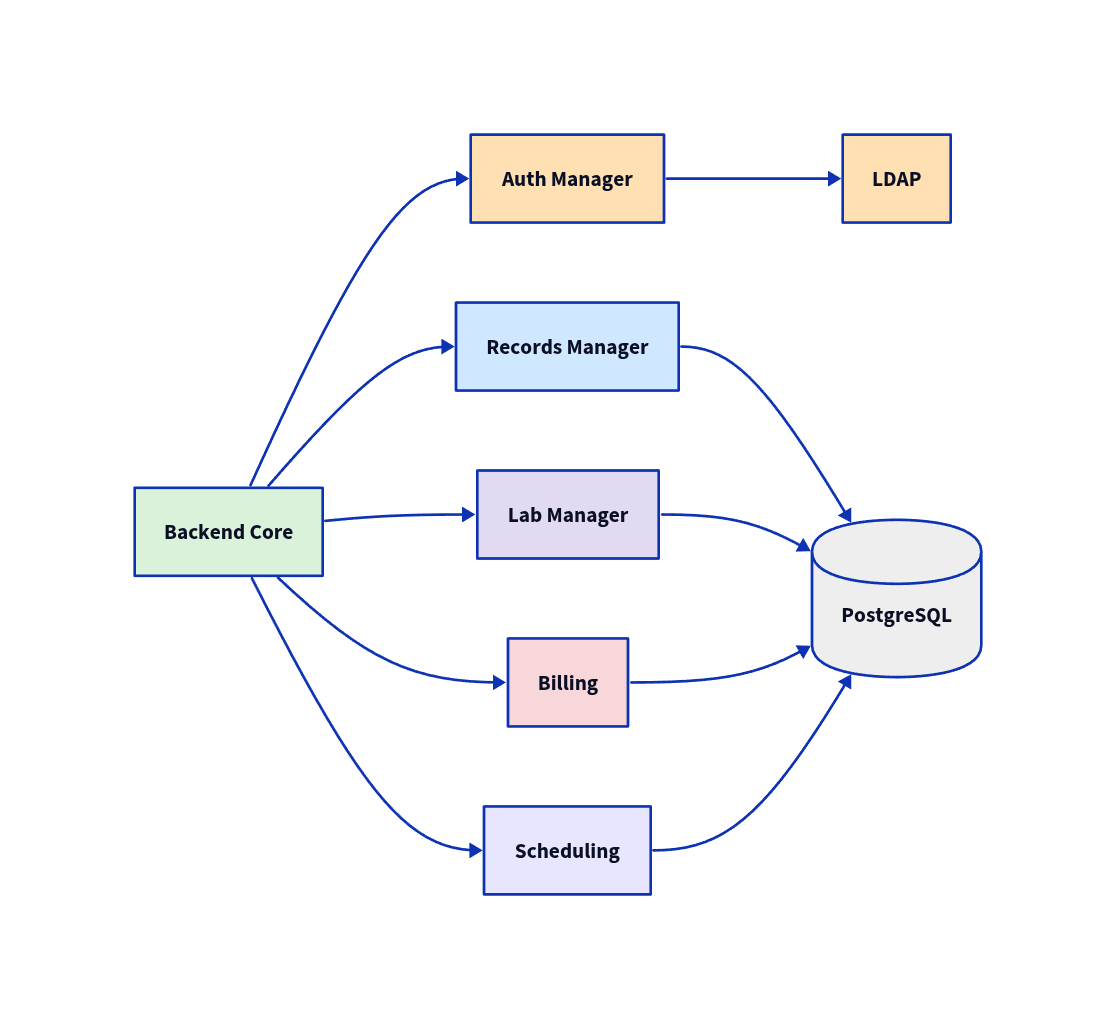
\includegraphics[width=\columnwidth]{figures/component-architecture.png}
\caption{Component-level decomposition supporting the chosen modular monolith architecture.}
\label{fig:components}
\end{figure}

\section{Results and Observations}
\subsection{Implementation Status Achieved}
The most important result after Assignment 1 is that the project is no longer only a requirements-and-diagrams exercise. The current repository contains:
\begin{itemize}
    \item a backend Express application exposing more than fifty documented API routes across authentication, visits, labs, billing, check-in, documents, events, and admin flows,
    \item a Prisma schema covering identity, visits, prescriptions, lab workflow, pharmacy, billing, attendance, events, and external documents,
    \item an idempotent seed script for role-specific users,
    \item a Bruno API collection organized by module,
    \item an executable smoke test script spanning the implemented backend together with a full end-to-end HTTP flow runner,
    \item and a minimal frontend scaffold awaiting actual dashboard development.
\end{itemize}

This asymmetry between backend maturity and frontend immaturity is itself an important result. It shows that the team prioritized the risk-heavy layers first: persistence, business rules, and route security.

\subsection{Implemented Module Coverage}
The delivered backend can also be understood as a set of working operational modules rather than only a count of routes. Table \ref{tab:modules} summarizes the state of the major modules visible in the repository.

\begin{table}[H]
\centering
\caption{Current Module Coverage}
\begin{tabular}{|p{2.05cm}|p{4.55cm}|p{1.15cm}|}
\hline
\textbf{Module} & \textbf{Delivered Capability} & \textbf{Status} \\
\hline
Authentication & Login, current-user resolution, JWT guarding, RBAC middleware & Working \\
\hline
Patient records & Self-profile, QR lookup, staff access, visit history & Working \\
\hline
Visit lifecycle & Create, vitals, claim, consultation, complete, cancel, queue & Working \\
\hline
Doctor operations & Availability, attendance, schedule views, doctor listing & Working \\
\hline
Prescription & Create, retrieve, pending queue, dispense & Working \\
\hline
Laboratory & Request tests, pending queue, report upload, patient access & Working \\
\hline
Medicine / billing & Inventory, stock update, bill generation, payment queue & Working \\
\hline
Appointments & Book, list, cancel, emergency override logic & Working \\
\hline
Check-in & QR-based visit creation with optional vitals & Working \\
\hline
Documents & Upload and list external records & Working \\
\hline
Admin / reports / notifications & User management, events, usage and attendance reports, physician-absence notifications & Working \\
\hline
Frontend dashboards & Role dashboards and UX integration & Not started \\
\hline
\end{tabular}
\label{tab:modules}
\end{table}

\subsection{Execution-Time Evidence from Current Artifacts}
The testing artifacts contain actual timing evidence rather than only projected estimates. The SRS states that standard user operations should return within a few seconds under normal load. The measured results satisfy that expectation with substantial margin.

\begin{table}[H]
\centering
\caption{Representative Measured Performance Results}
\begin{tabular}{|p{2.1cm}|p{2.7cm}|p{1.3cm}|p{1.3cm}|}
\hline
\textbf{Test ID} & \textbf{Operation} & \textbf{Threshold} & \textbf{Observed} \\
\hline
TC-P-001 & Login & 3000 ms & 77 ms \\
\hline
TC-P-002 & Patient profile retrieval & 3000 ms & 233 ms \\
\hline
TC-P-003 & Prescription retrieval & 3000 ms & 1215 ms \\
\hline
TC-P-004 & Atomic bill generation & 5000 ms & 1151 ms \\
\hline
TC-P-005 & Atomic QR check-in & 3000 ms & 796 ms \\
\hline
TC-R-001 & Login repeatability (15 runs, avg) & 3000 ms & 81 ms \\
\hline
TC-R-002 & Patient profile repeatability (15 runs, avg) & 3000 ms & 271 ms \\
\hline
TC-R-003 & QR check-in repeatability (15 runs, avg) & 3000 ms & 889 ms \\
\hline
\end{tabular}
\label{tab:perf}
\end{table}

Across the 48 rows currently recorded in \texttt{test\_cases.csv}, the observed overall mean response time is approximately 488.65 ms, with the slowest recorded value at 1291 ms. Even the heavier operations such as billing and prescription retrieval remain well within the SRS's ``few seconds'' expectation.

\subsection{Positive Results}
Several positive findings stand out:
\begin{itemize}
    \item \textbf{Traceability is no longer hypothetical.} The schema and services now physically enforce visit-linked relationships across the main clinical modules.
    \item \textbf{RBAC is operational.} Negative test cases show expected denials for unauthorized roles attempting protected actions such as bill generation or pharmacy queue access.
    \item \textbf{Atomicity is implemented where it matters.} Billing and QR check-in were not left as optimistic multi-step flows.
    \item \textbf{Administrative scope expanded successfully.} Sprint 5 work includes user management, PHC event publication, reporting, lab-request detail access, patient lab-report retrieval, and in-app doctor-availability notifications.
    \item \textbf{Testing maturity improved after Assignment 1.} The project now includes a repeatable smoke workflow and explicit timing evidence instead of only projected claims.
    \item \textbf{Authentication maturity improved.} The project moved from an LDAP design placeholder to a working local LDAP-backed bind flow used by tests and development setup.
\end{itemize}

\subsection{Negative Results and Corrective Observations}
The current state also exposes limits and negative findings that improved the team's understanding of the project:
\begin{itemize}
    \item \textbf{Production-grade identity integration is still incomplete.} Local LDAP-backed development is working, but real institutional rollout, credential lifecycle, and deployment security still need separate validation.
    \item \textbf{Frontend delivery was underestimated.} The README still lists Sprint 6 dashboards as not started, and the React application remains a placeholder. This forced a clearer separation between backend completion and user-interface completion.
    \item \textbf{Project artifacts need synchronization discipline.} The test guide mentions 53 cases, the smoke suite enumerates 56 identifiers, and the CSV ledger records 48 measured rows. This does not invalidate the backend, but it demonstrates a real documentation-maintenance problem.
    \item \textbf{Operational quality now depends on integration, not just coding.} The remaining blockers are less about writing another route and more about closing gaps among LDAP, staging migration, end-to-end validation, and frontend consumption.
\end{itemize}

\subsection{Artifact Consistency as a Project Result}
An unexpected but important result is that the project now contains enough engineering surface area for artifact consistency itself to matter. The available documents and scripts do not all describe the same testing state.

\begin{table}[H]
\centering
\caption{Observed Documentation and Testing Drift}
\begin{tabular}{|p{2.55cm}|p{3.45cm}|p{1.45cm}|}
\hline
\textbf{Artifact} & \textbf{Observed Count / Claim} & \textbf{Interpretation} \\
\hline
\texttt{TESTING.md} & states 53 automated cases & partially updated guide \\
\hline
\texttt{test\_cases.csv} & contains 48 measured rows & recorded evidence subset \\
\hline
\texttt{smoke\_test.sh} & enumerates 56 test IDs & latest executable scope \\
\hline
\end{tabular}
\label{tab:drift}
\end{table}

This observation is valuable because it reveals a practical engineering challenge that was not obvious at the start of the project: once the system has enough working parts, keeping the surrounding evidence synchronized becomes part of the deliverable.

\subsection{Requirement-to-Implementation Traceability}
The project now has enough implemented surface area for a compact traceability view to be meaningful. Table \ref{tab:traceability} summarizes how a few high-value requirements now map to concrete delivered behavior.

\begin{table}[H]
\centering
\caption{Compact Traceability Matrix}
\begin{tabular}{|p{0.95cm}|p{3.1cm}|p{2.1cm}|p{1.0cm}|}
\hline
\textbf{REQ} & \textbf{Delivered Behavior} & \textbf{Implementation Anchor} & \textbf{Sprint} \\
\hline
REQ-6 & LDAP-oriented authentication design & Auth service / config & 1 \\
\hline
REQ-15 & QR-based patient identification & Patient QR lookup, check-in route & 4 \\
\hline
REQ-22 & Claimed consultation ownership & Visit claim service & 2 \\
\hline
REQ-28 & Visit-linked traceability & Prisma visit relations & 2 \\
\hline
REQ-35/38 & Doctor attendance and checkout hours & Doctor attendance module & 2 \\
\hline
REQ-44/46 & Prescription creation and dispense flow & Prescription routes and services & 3 \\
\hline
REQ-54/55 & Lab request and report upload & Lab routes and services & 3 \\
\hline
REQ-64/66 & Billing plus inventory update & Billing transaction, medicine stock & 4 \\
\hline
REQ-49/52 & Admin user and reporting capability & Admin routes and report service & 5 \\
\hline
\end{tabular}
\label{tab:traceability}
\end{table}

\subsection{Module-Level Timing Interpretation}
The CSV evidence also makes it possible to compare average response behavior by module. This is useful because it distinguishes lightweight identity and profile operations from the heavier composite workflows that traverse more relations and business rules.

\begin{table}[H]
\centering
\caption{Selected Module-Wise Average Response Times from \texttt{test\_cases.csv}}
\begin{tabular}{|p{2.2cm}|p{1.4cm}|p{2.7cm}|}
\hline
\textbf{Module} & \textbf{Average} & \textbf{Interpretation} \\
\hline
Auth & 171.0 ms & lightweight identity operations \\
\hline
Patient & 263.2 ms & profile retrieval and updates remain fast \\
\hline
Visit & 310.4 ms & queue and lifecycle actions are efficient \\
\hline
Billing & 662.29 ms & heavier due to transaction and stock logic \\
\hline
Checkin & 680.75 ms & patient resolution plus visit creation work \\
\hline
Prescription & 748.57 ms & relation-heavy clinical retrieval and creation \\
\hline
Lab & 740.0 ms & upload and request operations are moderately heavy \\
\hline
Appointment & 586.75 ms & validation-heavy but still sub-second \\
\hline
\end{tabular}
\label{tab:moduleavg}
\end{table}

\subsection{Theory Versus Implementation Corrections}
One of the strongest outcomes of the project is that several theoretical assumptions from the earlier stages were refined after implementation:

\subsubsection{Sprint Structure}
The SRS proposed five implementation sprints. The current README expands the plan into seven slices, separating frontend and stabilization into dedicated later phases. This correction improved realism. It acknowledges that ``system integration'' in a healthcare workflow is not equivalent to ``system finished''.

\subsubsection{Performance Expectations}
The SRS described performance qualitatively. The actual backend now shows sub-1.3-second behavior across recorded measurements, allowing the team to replace vague assumptions with concrete evidence. In particular, the QR check-in flow, which was expected to materially reduce reception effort, is measured at 796 ms in one NFR run and 889 ms average across repeatability trials.

\subsubsection{Data-Model Confidence}
The earlier report argued that a relational model was preferable for PHC traceability. The implemented Prisma schema strengthens that conclusion. Prescriptions, lab reports, bills, vitals, doctor attendance, and documents now coexist in a model where referential integrity is inspectable and testable rather than only architecturally claimed.

\subsection{Operational Factors Identified Late}
Some debilitating factors became clear only after implementation work started:
\begin{itemize}
    \item \textbf{Development conveniences can still hide deployment risk.} Even though local LDAP-backed development is now working, institute-grade rollout, credential lifecycle handling, and deployment security still require separate validation.
    \item \textbf{Testing evidence itself becomes an artifact to maintain.} Once the project gained automated checks, consistency between scripts, CSV logs, and narrative docs became necessary.
    \item \textbf{User-interface absence limits stakeholder validation.} Even with a working backend, a PHC stakeholder will still perceive the product as incomplete until role dashboards exist.
\end{itemize}

\subsection{Novelty and Comparative Advantage}
The project should not overclaim against the global state of the art; no formal benchmark against commercial hospital platforms has been conducted. However, relative to generic appointment tools and heavyweight hospital systems, the design does exhibit practical novelty in its target context:
\begin{itemize}
    \item \textbf{Institution-specific identity integration:} the design is anchored around IIT Jodhpur credentials rather than creating a separate credential universe.
    \item \textbf{Unified outpatient traceability:} check-in, consultation, prescription, lab, billing, and documents are handled in one visit-centric model.
    \item \textbf{Lightweight deployability:} a modular monolith is better matched to a campus PHC than an enterprise hospital stack or a fragmented set of standalone tools.
    \item \textbf{Administrative observability:} attendance, reports, and event management are treated as first-class system concerns rather than afterthoughts.
\end{itemize}

\begin{figure}[H]
\centering
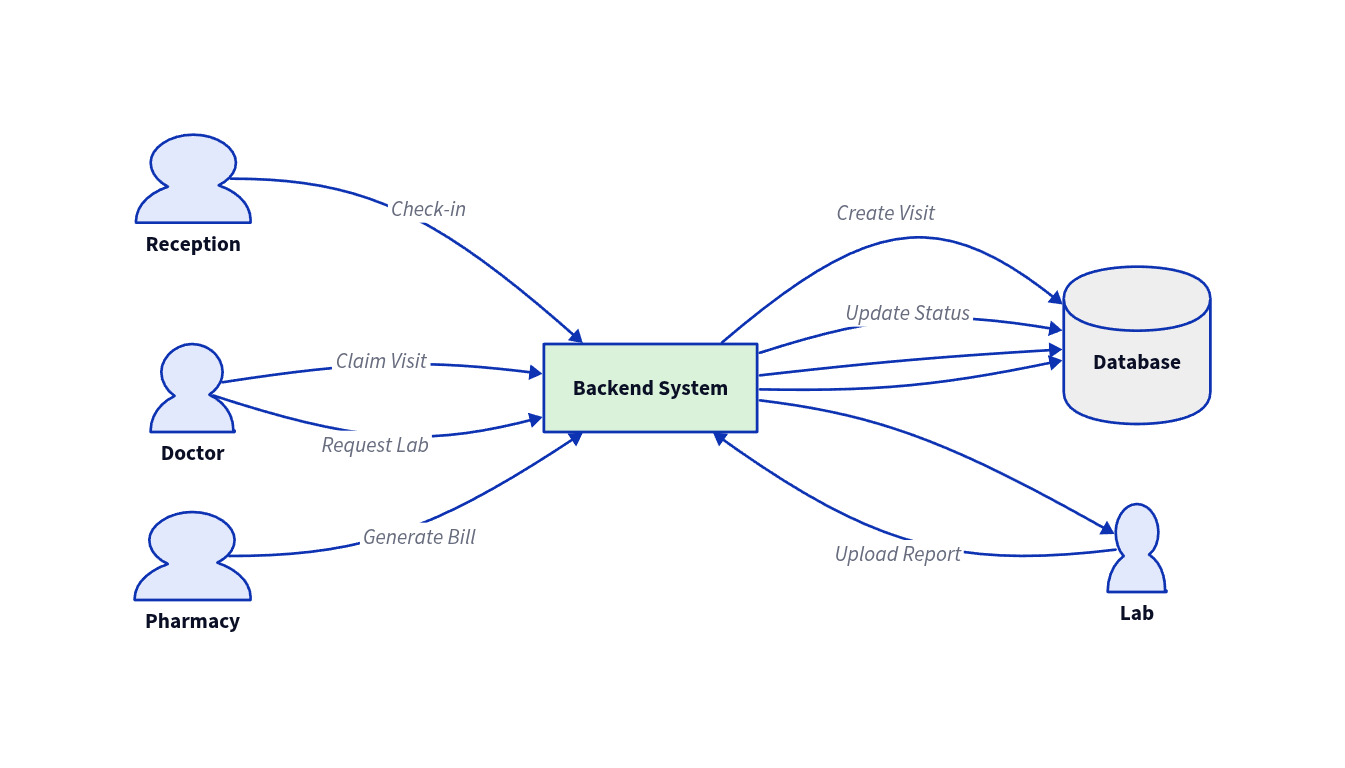
\includegraphics[width=\columnwidth]{figures/end-to-end-visit-lifecycle.png}
\caption{End-to-end patient-flow model retained as a valid summary of the working backend's intended operational path.}
\label{fig:lifecycle}
\end{figure}

\subsection{Current Project Position}
As of April 5, 2026, the clearest defensible conclusion is that the PHC Integrated Digital System has crossed the line from conceptual architecture to a functionally rich backend platform. Sprint 5 backend integration is effectively closed, and the remaining risks are now concentrated in frontend completion, integration hardening, documentation consistency, and institutional deployment details rather than in basic system design.

\section{Discussion}
\subsection{Security and Privacy Implications}
Healthcare systems must be evaluated not only by functionality but by whether access boundaries are enforceable. The current backend already demonstrates several positive security-oriented properties: authenticated access for non-public routes, role-gated authorization, centralized error handling, response normalization, and request-surface protection through middleware such as \texttt{helmet}.

At the same time, the repository clarifies what is still pending before a production interpretation would be justified. Stronger auditability, HTTPS deployment enforcement, institutional identity rollout, and operational secrets discipline belong to the remaining hardening work. This distinction is important because the project already reflects a secure design direction even though the deployment-grade security story is incomplete.

\subsection{Why the Chosen Design Still Holds}
The implemented repository strengthens the original argument for a modular monolith. A three-member team was able to deliver a broad backend, preserve module boundaries, and maintain testability without the operational complexity of distributed services. The design therefore appears well matched to an institute PHC where maintainability and low deployment friction matter more than premature service decomposition.

\subsection{What Assignment 2 Changed in Team Understanding}
The most important change since Assignment 1 is epistemic: the project is no longer judged only through diagrams and projected benefits. It now produces empirical feedback. Route behavior, timing measurements, negative-case failures, unfinished integration points, and documentation drift all provide concrete evidence that shapes the next iteration. That shift from modeled confidence to observed confidence is one of the strongest educational outcomes of the project.

\section{Conclusion}
The Assignment 2 state of the PHC Integrated Digital System shows meaningful convergence between requirements, architecture, and implementation. The team has preserved the strongest ideas from Assignment 1 and SRS 2.0, especially role-based access, visit-linked traceability, QR-assisted reception flow, and modular separation of concerns, while also correcting earlier assumptions through concrete implementation work.

The results are mixed in the right way. The backend demonstrates substantial functional progress, working LDAP-backed development authentication, and encouraging performance behavior, but the project also reveals absent production-grade frontend dashboards and the maintenance burden of keeping testing and documentation artifacts synchronized. These are not signs of conceptual failure; they are signs that the project has moved into the integration-heavy phase where disciplined engineering matters more than broad ideation.

For the PHC context at IIT Jodhpur, the project is already strong as a backend-centered digital foundation. The next decisive milestone is to close the loop among frontend usability, institutional authentication, end-to-end validation, and deployment readiness.

\section{AI Usage Declaration}
AI tools were used only for writing assistance, restructuring, and language refinement of this report. The technical basis of the report was derived from the repository contents, SRS 2.0 / 2.1 / 2.2, Assignment 1 artifacts, UML diagrams, and current implementation files. Architectural decisions, sprint structure, requirements framing, and implementation work remain the team's own project contributions.

\begin{thebibliography}{00}

\bibitem{b1} Y. Bavadiya, C. Singh, and N. Patidar, ``Software Requirements Specification for PHC Integrated Digital System, Versions 2.0, 2.1, and 2.2,'' IIT Jodhpur, Feb.--Apr. 2026.

\bibitem{b2} Y. Bavadiya, C. Singh, and N. Patidar, ``Design and Implementation of the PHC Integrated Digital System: A Modular Healthcare Architecture for IIT Jodhpur,'' Assignment 1 submission, IIT Jodhpur, Feb. 2026.

\bibitem{b3} ``PHC Integrated Digital System README,'' repository artifact, Mar. 2026.

\bibitem{b4} ``PHC System -- Testing Guide,'' repository artifact, Mar. 2026.

\bibitem{b5} ``PHC Integrated Digital System automated smoke test suite,'' \texttt{backend/smoke\_test.sh}, repository artifact, Mar. 2026.

\bibitem{b6} ``PHC Integrated Digital System test case ledger,'' \texttt{test\_cases.csv}, repository artifact, Mar. 2026.

\bibitem{b7} IEEE Computer Society, ``IEEE Recommended Practice for Software Requirements Specifications,'' IEEE Std 830-1998, 1998.

\bibitem{b8} K. Schwaber and J. Sutherland, ``The Scrum Guide,'' Scrum.org, Nov. 2020. [Online]. Available: \url{https://scrumguides.org/}

\bibitem{b9} PostgreSQL Global Development Group, ``PostgreSQL Documentation.'' [Online]. Available: \url{https://www.postgresql.org/docs/}

\bibitem{b10} Prisma Data, Inc., ``Prisma ORM Documentation.'' [Online]. Available: \url{https://www.prisma.io/docs/orm}

\bibitem{b11} OpenJS Foundation, ``Express -- Node.js web application framework.'' [Online]. Available: \url{https://expressjs.com/}

\bibitem{b12} M. Jones, J. Bradley, and N. Sakimura, ``JSON Web Token (JWT),'' RFC 7519, May 2015.

\bibitem{b13} OWASP Foundation, ``OWASP Application Security Verification Standard 4.0.3,'' 2021. [Online]. Available: \url{https://owasp.org/www-project-application-security-verification-standard/}

\end{thebibliography}

\clearpage
\appendices
\section{Final UML Diagrams}
The appendix reproduces the UML set carried forward from the SRS/Assignment 1 design baseline. These diagrams remain the best compact visual summary of the intended end-to-end system behavior and structural decomposition. If the course staff expects newer diagram revisions, insert them here in place of the inherited versions.

\begin{figure*}[!t]
\centering
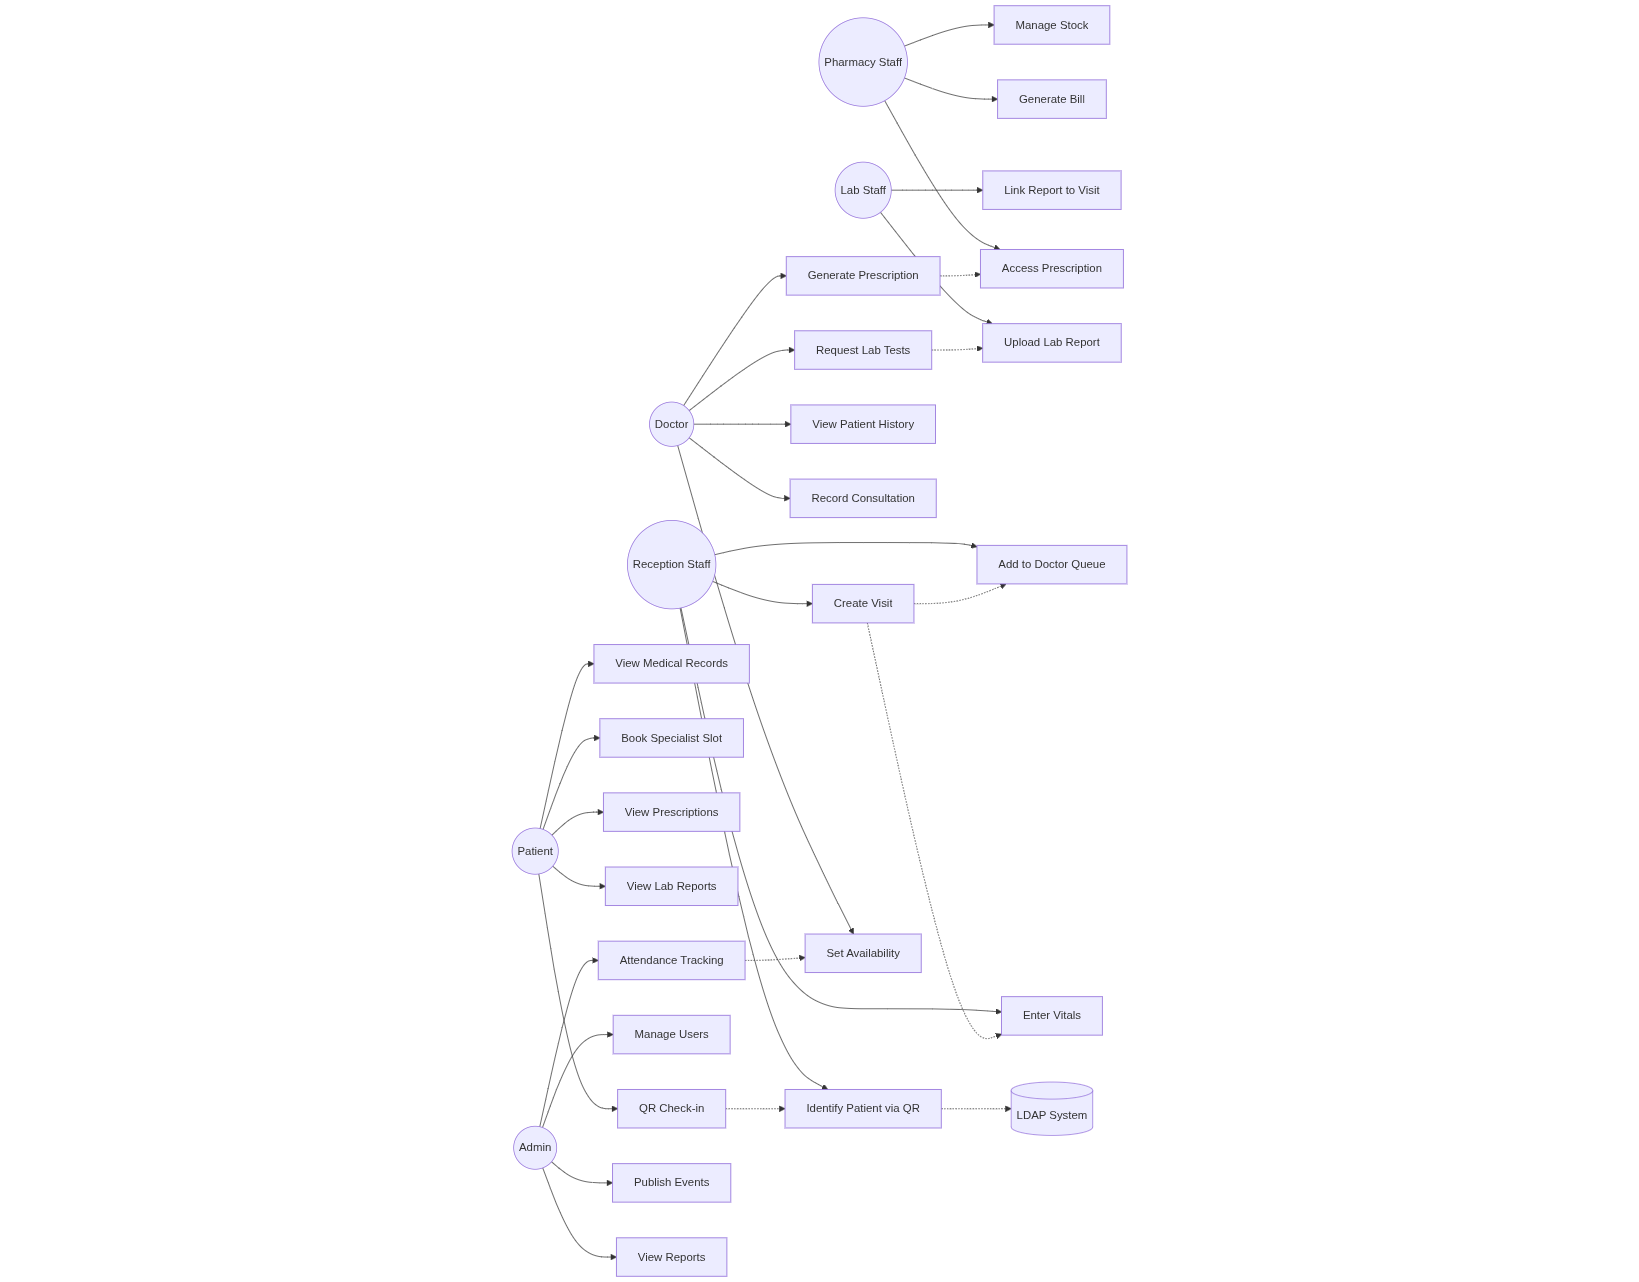
\includegraphics[width=0.92\textwidth]{figures/srs-use-case.png}
\caption{Use case diagram.}
\label{fig:srs-usecase}
\end{figure*}

\begin{figure*}[!t]
\centering
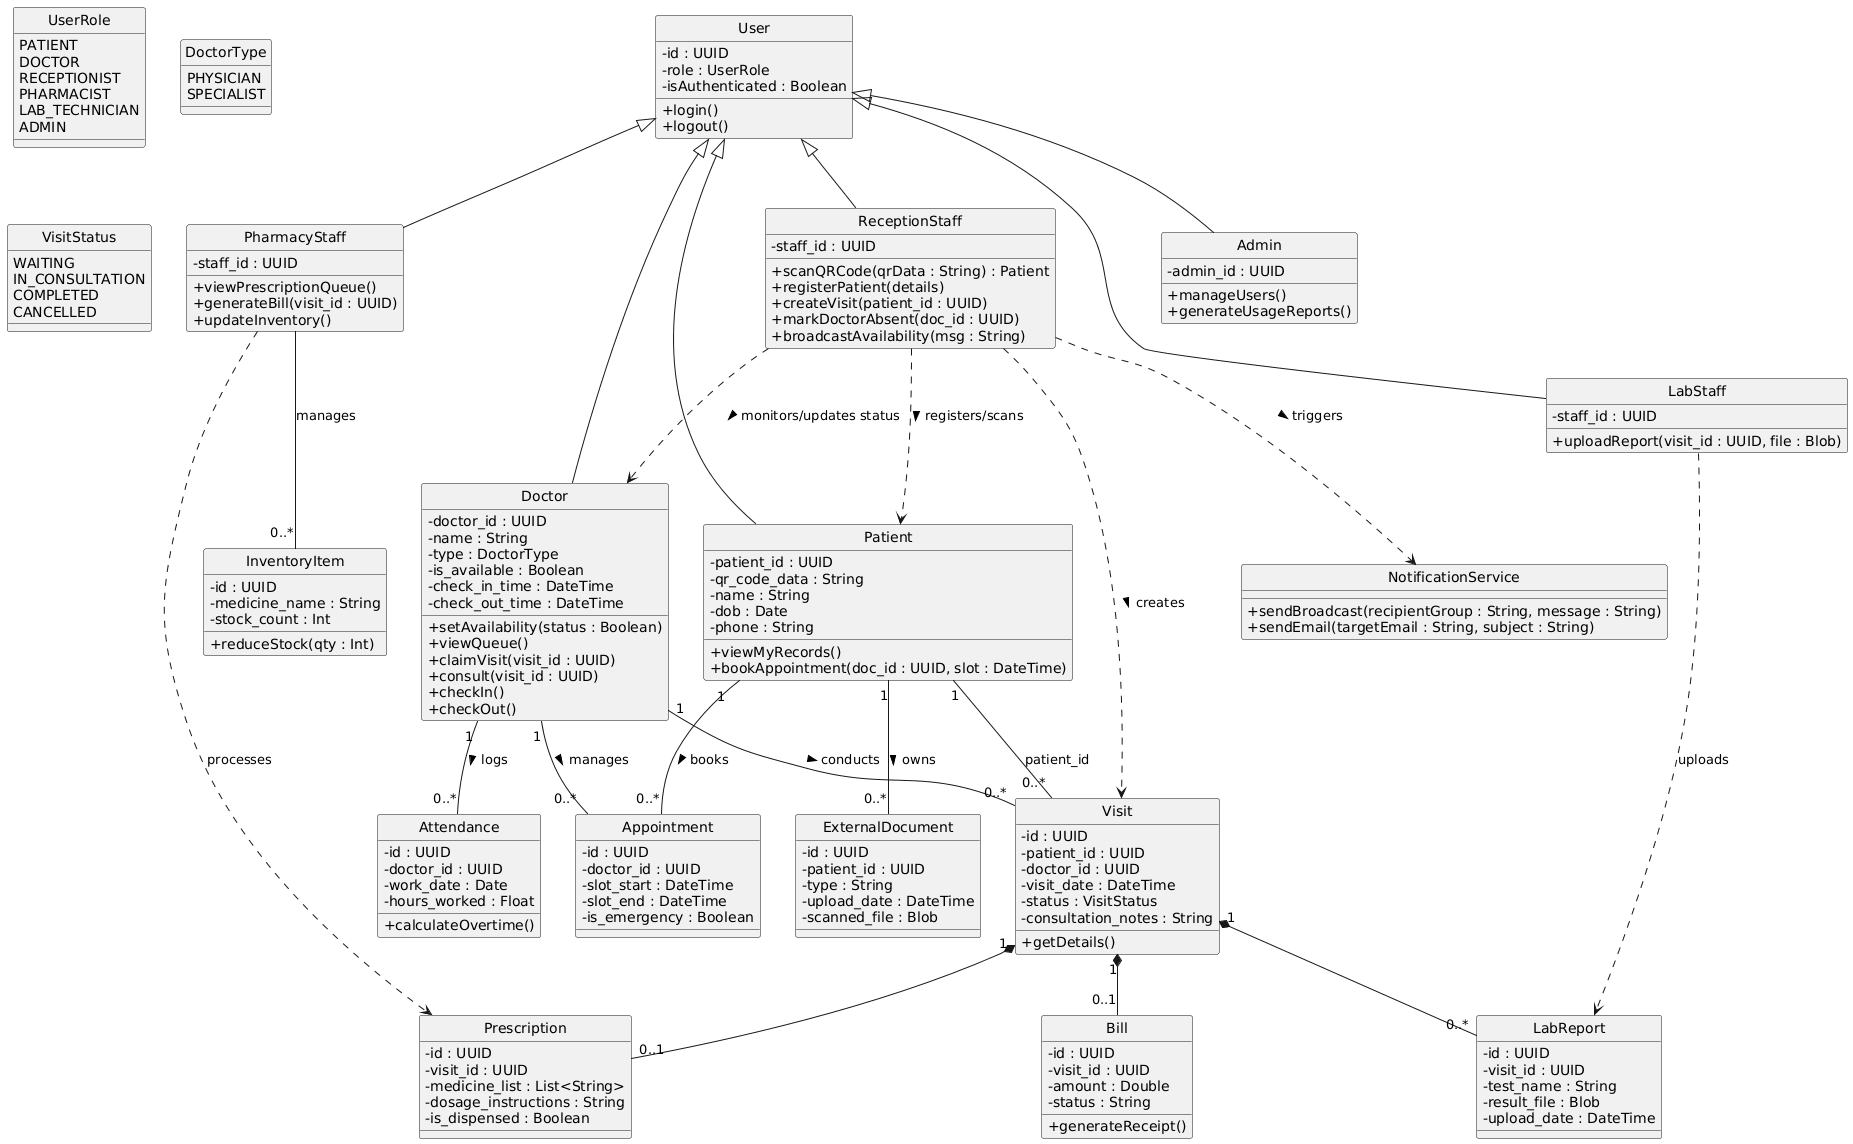
\includegraphics[width=0.92\textwidth]{figures/srs-class-diagram.png}
\caption{Class diagram.}
\label{fig:srs-class}
\end{figure*}

\begin{figure*}[!t]
\centering
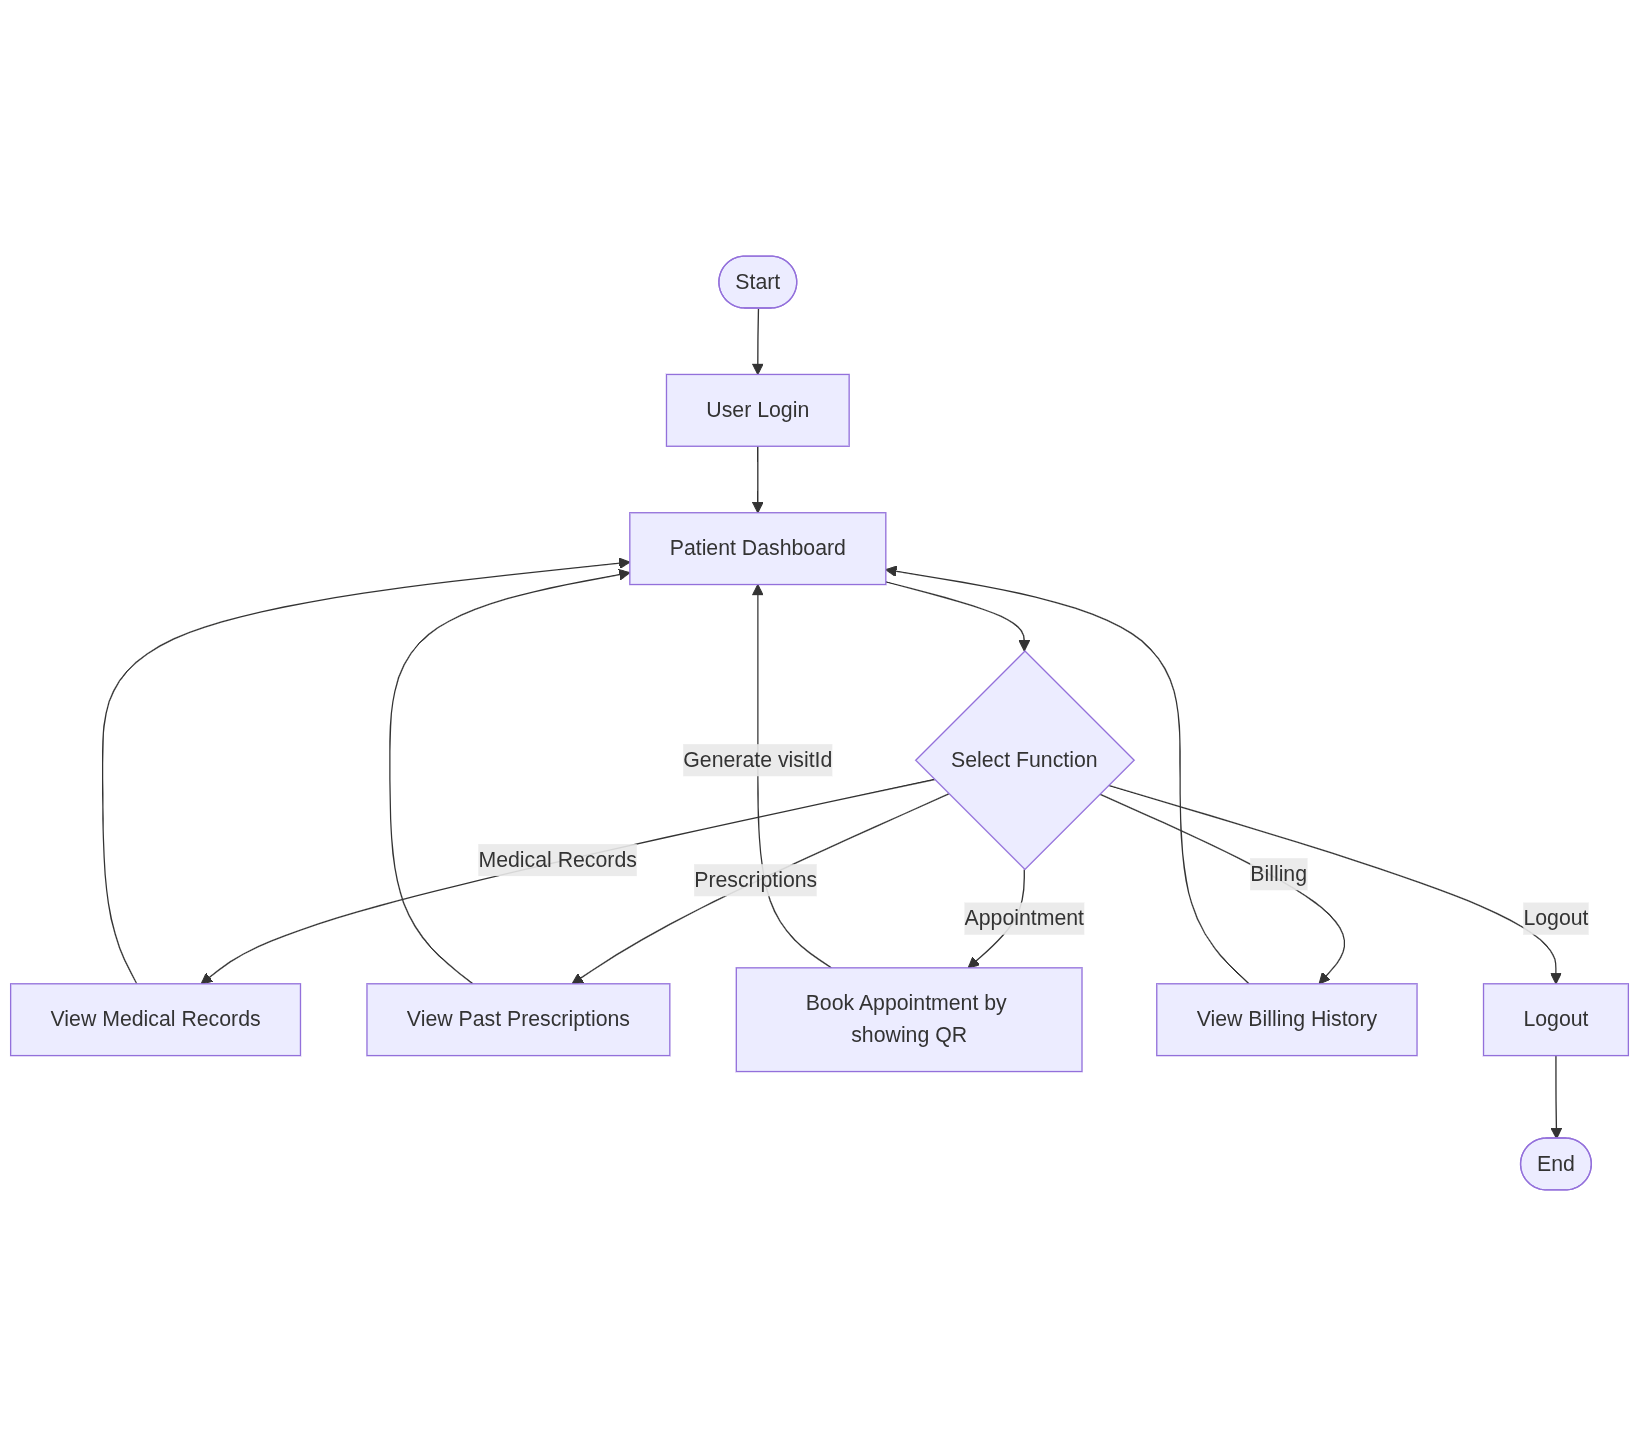
\includegraphics[width=0.92\textwidth]{figures/srs-patient-workflow.png}
\caption{Patient workflow activity diagram.}
\label{fig:srs-patient}
\end{figure*}

\begin{figure*}[!t]
\centering
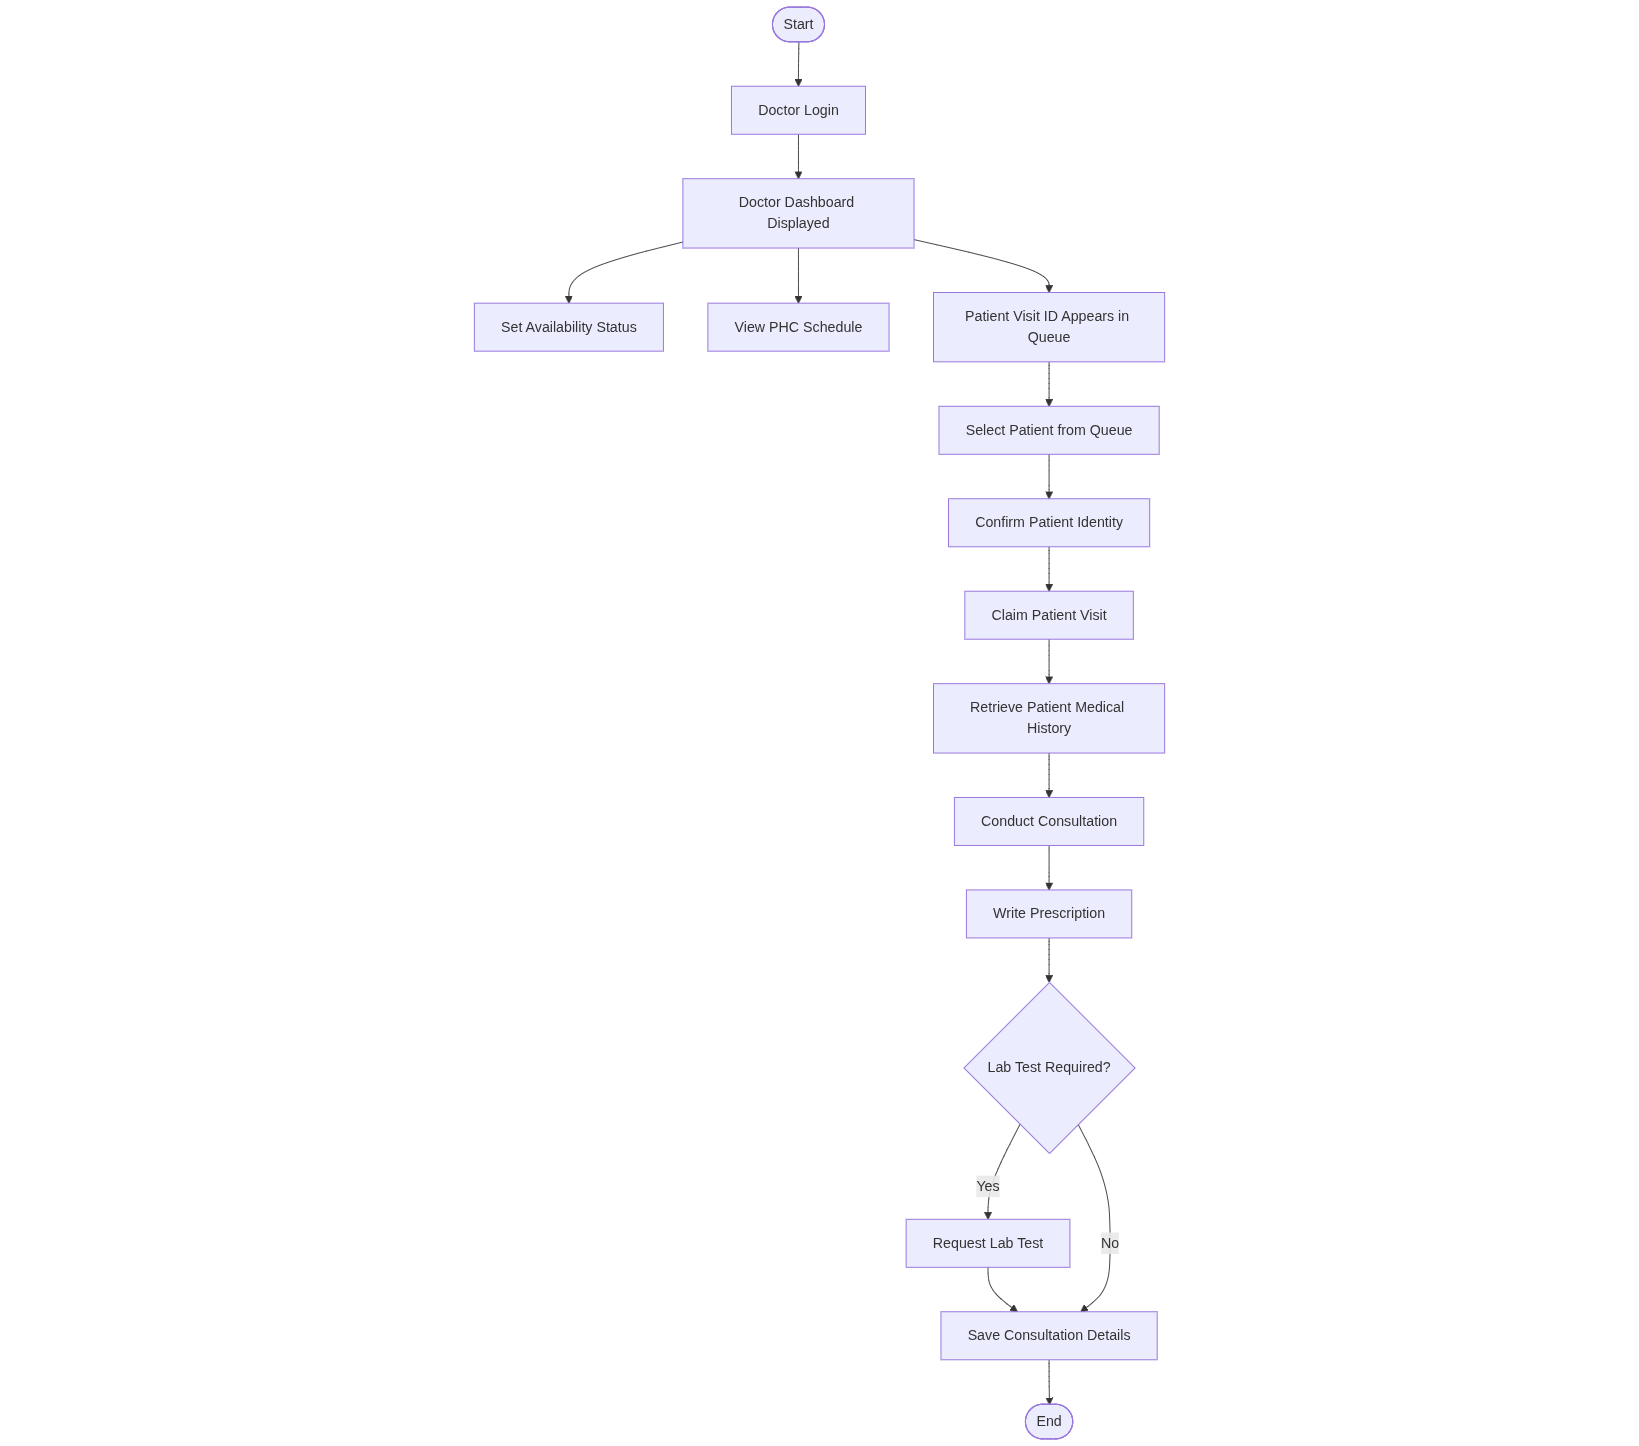
\includegraphics[width=0.92\textwidth]{figures/srs-doctor-workflow.png}
\caption{Doctor workflow activity diagram.}
\label{fig:srs-doctor}
\end{figure*}

\begin{figure*}[!t]
\centering
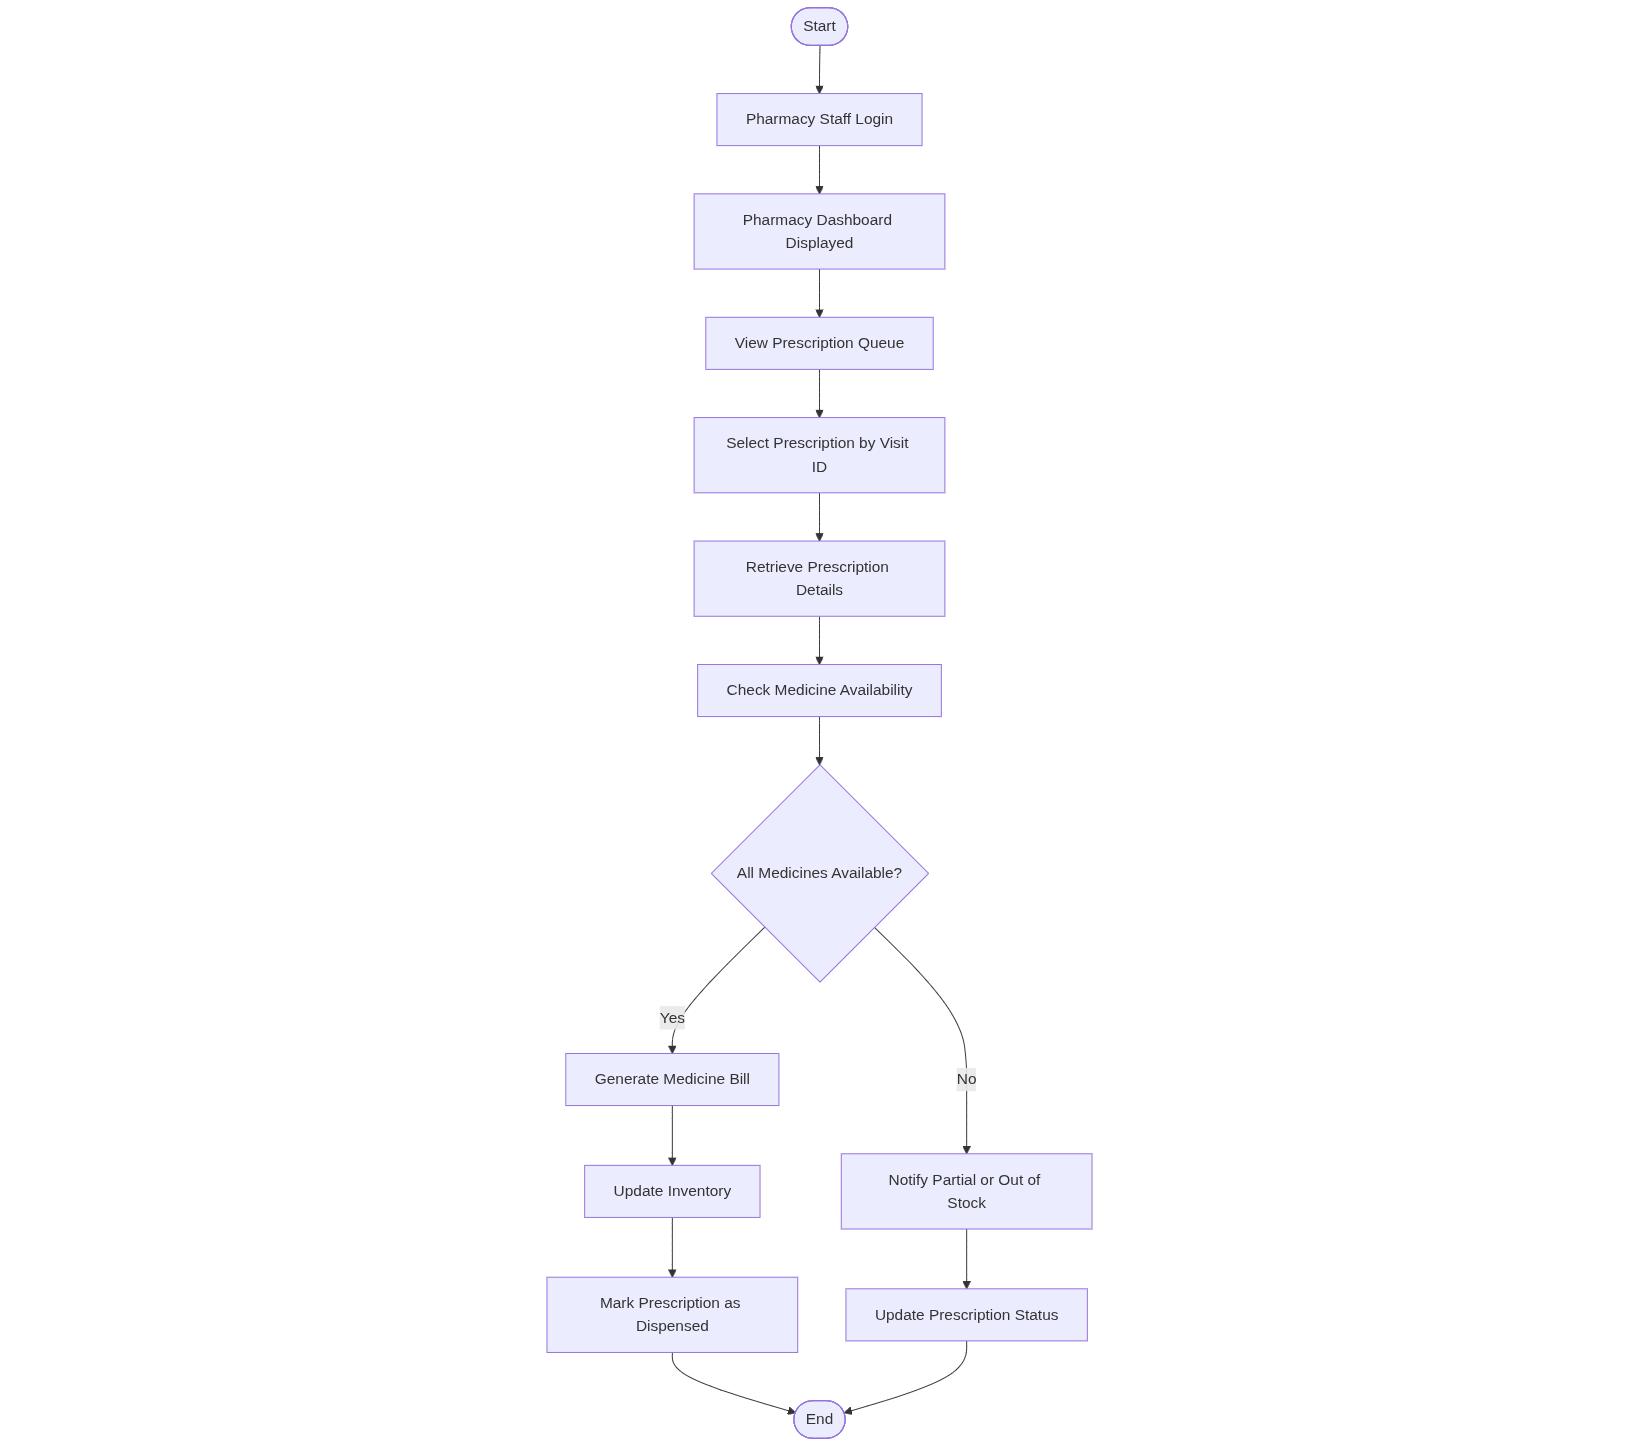
\includegraphics[width=0.92\textwidth]{figures/srs-pharmacy-workflow.png}
\caption{Pharmacy workflow activity diagram.}
\label{fig:srs-pharmacy}
\end{figure*}

\begin{figure*}[!t]
\centering
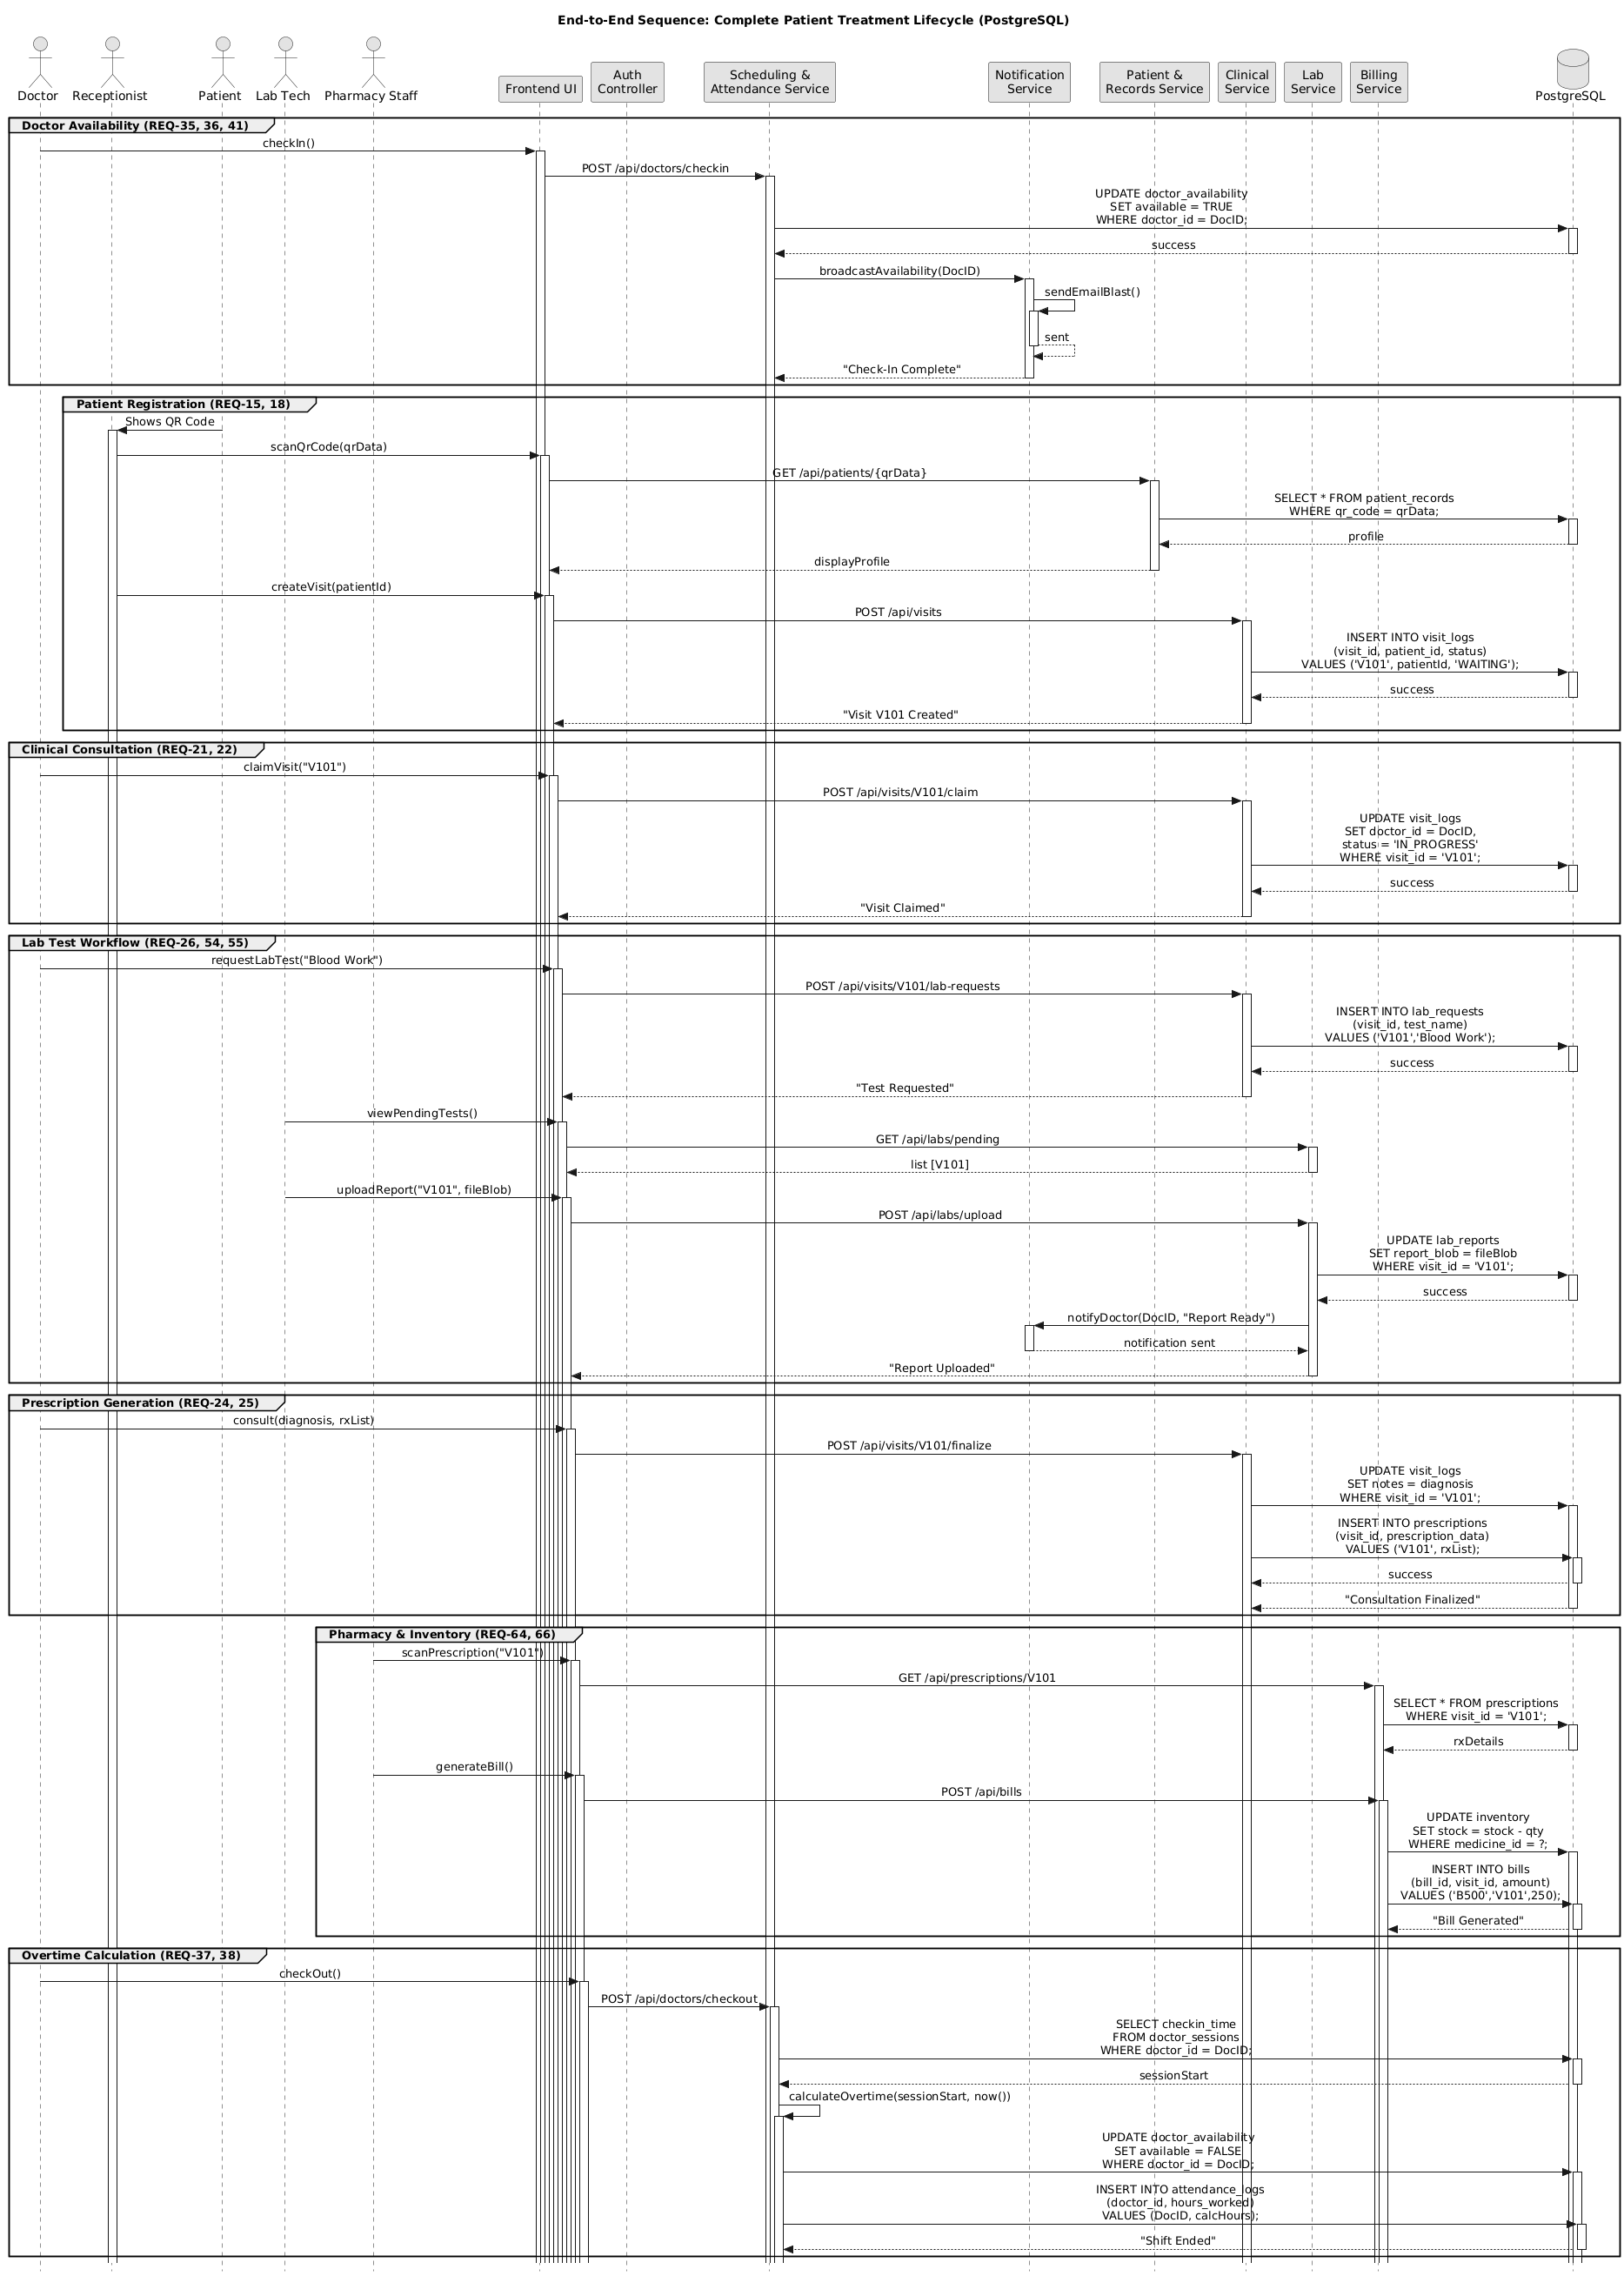
\includegraphics[width=0.92\textwidth]{figures/srs-sequence.png}
\caption{Sequence diagram.}
\label{fig:srs-sequence}
\end{figure*}

\end{document}
